\chapter{A Graph Theoretic Approach to U.S. Army Field Ration Menu Development}
\section{Abstract}
The graph theoretic approach to analyzing food combinations is based on pairwise compatibility information regarding pairs of items.  From this information, which can be collected directly from subjects in a straightforward manner, compatibility information for larger combinations is predicted.  This approach has been validated at the individual and group levels for meals consisting of combinations of items within a single category, but has not yet been applied to meals, such as boxed lunches, that are composed of representatives from distinct categories.  The study presented in this paper extends the graph theoretic approach to such a situation, specifically to military rations known as Meal-Ready-to-Eat or MREs\tm.  MRE\tm menus are composed of 11 different food categories (entr\'{e}e, side, snack, etc.) and there are multiple items available in each category.  From these items, over 22 billion potential menus can be formed.  To identify the most compatible of these menus, pairwise data regarding food item combinations across categories were collected from soldiers familiar with MREs\tm.  These soldiers were asked whether or not pairwise combinations of components were appropriate to combine in a meal.  Using graph theoretic tools, predictions were made of optimal MRE\tm menus and rankings, based on the pairwise information, were created to assist product developers in the improvement of existing menus and the invention of promising new menus.  By applying the graph theoretic approach to meals with multiple categories, and by implementing a ranking approach to assess the compatible menus identified by the graph theoretic technique, this paper adds two unique contributions to the growing body of literature on combinatorial tools in sensory and consumer science.

\section{Introduction}

Consumer driven approaches to menu development have been elusive.  A menu is classically defined as “The portion of food taken at a particular time for the satisfaction of appetite; the quantity usually taken at one time with the purpose of satisfying hunger; a repast” \citep{Webster1913}.  Thus, with regard to a single meal, the menu is the specific set of foods that comprise that meal.  Perhaps unsurprisingly, this definition does not capture the complexity of the meal experience nor give any indication of how to control it.  The food industry has not spent much effort developing meals, rather the focus has been on individual items \citep{Meiselman2000}.  \citet{Meiselman2000} notes that the reason for this gap is because of the complexity of the meal experience which is composed of social, psychological \citep[see esp.][chap. 2]{Lawless2010}  and nutritional factors.  For operational purposes then, we define a meal as a combination of foods from separate categories intended to be consumed together.  
An example menu for a typical southern American meal is smoked pork with barbeque sauce, corn bread, baked beans, coleslaw and lemonade.  The good “categories” in this example are protein, sauce, starch, bread, vegetable and drink respectively.  The reason that these items work well together to create a cohesive “southern American summer barbeque” concept is beyond the scope of this paper, but it includes all of the factors listed above - social: history and tradition, psychological: flavor contrasts \citep{Lawless1977,Lawless1979,Lawless1987,Lawless2010,Lawless2000} and nutritional: protein, fat, starch and a diverse array of nutrients.  The reader could easily come up with a favorite meal from their childhood and also note the complexity as to the reasons “why?” their favorite meal may be considered a good concept.   

When consumer scientists and researchers create meals for commercial production, it is often the complexity of the meal concept that drives development, not considerations of consumer liking.   Many foodservice manufacturers employ research chefs or use internal “experts” to make meal concept decisions.  Other sources for these concepts include teams of food scientists or the established literature.  All of these approaches are notable for the lack of utilizing the intended consumer of the product as a source of information on how the components should be combined together.  

Despite the challenges, there have been some attempts at consumer driven approaches.  Regression based approaches have been used to predict consumer preference for combinations of food items from the preference scores of the individual items \citep{Eindhoven1959,Hedderley1995,Moskowitz1995}.  Unfortunately predictions were poor due to combination effects that this approach neglects to account for, including consumer ethnicity, context, texture, color and frequency of consumption \citep{Eindhoven1959,Marshall2003,Niewind1986,Pilgrim1961}.  

Conjoint analysis is a more advanced regression approach, based on consumer responses, which has achieved some success in predicting consumer preference \citep{Green1978,Luce1964}.  Conjoint analysis predicts combinations by presenting multiple scenarios with different factor levels of the same factor (e.g. different entr\'{e}es or sauces) and finding utility scores for each factor level for its contribution to the overall concept.  Using this approach, an optimal concept or combination of concepts can then be predicted \citep{Moskowitz2006a}.  A more recent advancement in conjoint based approaches allows the consumers themselves to choose the factor levels in which they are interested from a list of alternatives \citep{Liechty2001}.

One notable soldier-based study gives insight into one of the reasons there are challenges with the regression based approaches.  In this study, a bartering metric was used to evaluate how soldiers perceived a meal compared to individual items \citep{Lawless1994}.  Soldiers were observed in the field trading meal items with each other, much as elementary children do during school lunches.  Often, soldiers would build up reserves of a favorite item to use as trading material.  In 1994 this item was the Desert Bar, a chocolate snack product.  Soldiers rated how many Desert bars that they would trade for individual items.  Next, they rated how many desert bars they would trade for an entire meal, composed of the items they had previously rated.  It was observed that the meal was worth less than the sum of the component parts on the “desert bar scale.”  This meal discounting effect has analogies in economics, where, for example, home audio theater systems are cheaper than purchasing separately speakers, a television and a DVD player.  By showing that this effect occurs in foods, Lawless showed that there may be economic-like forces that affect our evaluation of meals.  This discounting effect can be problematic for regression approaches that depend on additivity.  More generally, these challenges together with the complexity of regression based approaches lead us to a relatively new approach to predicting combinations of foods that can be combined to produce desirable meals.

\subsection{Graph Theory}

Graph theory is the mathematical study of connections \citep{Bollobaas1998}.  For our purposes, graph theory  provides a toolkit which, when applied to foods, provides a novel methodology for examining meal component combinations.  In this graph theoretic framework, foods are represented as vertices and foods to which they are connected as edges between them \citep{Ennis2011}.  The advantage of this representation is that it allows us to conduct advanced analyses on how the foods are psychologically connected.  

\citet{Ennisa} have provided a specific graph theoretic methodology for examining consumer responses and creating a cohesive model for predicting how items should be combined together If a consumer scientist is trying to create pizzas for a fixed-item menu at a large restaurant franchising chain, for example, she might have twenty-five toppings to choose from, and she also wants between three to eight toppings on the pizzas.  The exhaustive list of possibilities is 1,807,480 unique pizzas.  The graph theoretic model provides a consumer driven screening approach \citep{Ennis2011} in which this list is screened down to a small number of highly compatible pizzas.  In a typical scenario, this list would then go on to traditional methods of choosing a final list of pizzas to be introduced.  The advantage is that this approach screens out close to two million pizzas, an impossible feat by any other typical product development scenario.  

In the \citet{Ennisa} model, consumers are presented with a list of pairwise combinations of food items and asked whether or not it would be appropriate to combine the two items together.  This unique approach, essentially, fills in the edges of a graph.  Graph theoretic algorithms can then be applied to the responses to predict larger combinations of items.  For example, if a consumer states that the combinations Peach-Vanilla, Vanilla-Orange and Peach-Orange are compatible flavors as pairs, then the larger combination Peach-Vanilla-Orange is a predicted compatible combination.  This larger combination is known as a clique, defined as a completely connected set of vertices \citep{Moon1965}.  However, if one of the pairs, such as Peach-Orange is not compatible, then the larger combination is not compatible.  This concept of seeking fully compatible combinations easily scales up to larger combination sizes depending upon goals.  

This approach was first applied to foods by \citet{Nestrud2010a} in an examination of salad components.  The purpose of the salad study was to highlight and validate the \citet{Ennis2010} approach by presenting consumers with all possible pairs of twenty-five salad ingredients and ask whether or not they thought it would be appropriate to combine the components together on a salad.  Predicted salads of size three to eight were created for each individual based on their responses.  Subjects were then asked whether or not the predicted salads, as well as a selection of random combinations that were predicted to be incompatible (e.g. at least one pair was not connected for the subject), were in fact compatible.  Overwhelmingly, for all combination sizes three through eight, the results supported the compatibility (as measured by appropriateness) of the predicted combinations over the random combinations, thus validating the graph theoretic approach.

\subsection{Meal-Ready-To-Eat or MREs}

The purpose of the MRE\tm, or Meal, Ready to Eat\tm is to provide US military personnel with nutritional sustenance where food service facilities are not available.  Three MREs\tm provide a day’s worth of subsistence.  Each ration is small and portable, occupying no more than 0.08 ft\superscript{3}.   The components of an MRE\tm include an entr\'{e}e, starch, spread, dessert, snacks, bakery item, fruit and a condiment.  Twenty four different MREs\tm are in rotation at any given period and from 1993 through 2010, 216 new items were added to menus and 65 removed \citep{RDECOM2010}.  One of the challenges of development is deciding what existing food items to pair with items that are being considered for introduction.  MRE\tm development is the responsibility of the Combat Feeding Directorate of the U.S. Army Natick R,D and E Center under the authority of the United States Department of Defense.

It has been noted that the “development of new combat rations is fueled by the wants, needs and ideas of Warfighters themselves” \citep{RDECOM2010}.  However, due to complexities of defining meal concepts noted above the primary focus of research has been on the development of individual ration components.  Soldiers provide acceptability information on individual items, and perhaps entire meal concepts, but there has not been a soldier-centric approach to deciding what components best go together to form a meal.  One of the major reasons for this is that there are 22,140,518,400 potential MREs\tm that can be created from the available components!  The current approach is for a small team to decide on which components should be combined, and then these concepts are approved by both soldier surveys and by Department of Defense officials.  Generalizing the graph theoretic approach to our present purposes, however, we propose a new approach for streamlining this type of menu development using input from consumers, who in this case are soldiers.

In this paper then, we present the results of a study designed to extend the graph theoretic screening method of \citet{Ennisa} to more complex food items such as MREs\tm.  In these more complex items, there are inherent restrictions as the combinations being screened are composed of items from many different categories.  In the case of the MRE\tm, for example,  there are eleven different categories and only one item per category is utilized. This restriction has a number of implications for both the experimental design and analysis.  Extending the graph theoretic approach to this restricted environment, we will predict most compatible menus, including two never-before-seen entr\'{e}es.  In addition, we introduce a novel concept of ranking for the candidate menus based on overall compatibility, which enhances previous approaches by not only providing a list of highly compatible menus, but also by providing information that predicts the relative performance of the proposed menus.  

\subsection{Experimental Overview}
The present investigation uses a complex meal item, the MRE\tm, which is composed of eleven categories of food items with many choices of items for each category, and utilizes a graph theoretic optimization strategy to predict most compatible MRE menus..  The concept of appropriateness \citep{Schutz1988} provides us the framework for conducting our study under the correct context.  In particular, we use appropriateness to connect the graph theoretic framework  to the meal experience variables mentioned by \citet{Meiselman2000} (e.g. social and psychological).  To these ends, our primary consumers, military personnel, were recruited on-site in Fort Drum, NY to answer surveys about menu items.  The graph theoretic tools were applied to the responses and ranked MRE\tm menus were presented to the Combat Feeding Directorate for final consideration.

\section{Materials and Methods}
\subsection{Subjects}
Two hundred and seventy active duty personnel (216 male) were recruited at Fort Drum, New York, USA to take part in the survey.  These soldiers comprised a convenience sample of primary consumers.  Their average age was 26 and most of them had been in the armed forces for at least five years.  All had previous experience with MREs\tm and 115 had eaten them at least once in the past six months.  

\subsection{Survey Design}
Eleven different categories of components were considered for evaluation and are listed in Table\ref{tab:mrefood}.

\begin{landscape}
\footnotesize
\begin{longtable}{p{7cm}p{7cm}p{7cm}}
\caption{Categories and MRE\tm items currently available to the Combat Feeding group.} \\
\label{tab:mrefood} \\
\toprule
\endfirsthead
\toprule
\endhead
\midrule
\multicolumn{3}{c}{Continued on next page...} \\
\endfoot
\bottomrule
\endlastfoot
\multicolumn{3}{l}{\bf Entrees} \\
\cmidrule(l){1-1}
Beef Patty, Jalapeno Pepper Jack & Beef Ravioli in Meat Sauce & Beef Roast with Vegetables\\
Beef Stew & Beef Taco Filling & Brisket Entree \\
Cheese Tortellini in Tomato Sauce & Chicken Fajita & Chicken Marsala \\
Chicken, Noodles and Vegetables in Sauce & Chicken Pesto Pasta & Chicken, Pulled with Buffalo Sauce \\
Chicken with Tomatoes and Feta & Chili and Macaroni & Chili and Beans \\
Maple Sausage Wrap & Meatballs in Brown Gravy & Meatballs in Marinara Sauce\\
Mexican Style Chicken Stew & Penne with Veg. Sausage, Spicy Tom. Sce. & Pork Rib, Boneless\\
Pork Sausage Patty, Maple Flavored & Pork Sausage with Gravy & Ratatouille\\
Sloppy Joe Filling & Southwest Style Beef and Black Beans & Spaghetti with Meat and Sauce \\
Spicy Sweet and Sour Pork, Shredded & Szechuan Vegetables and Tofu & Tuna, Lemon Pepper \\
Turkey Chili with Hominy & Vegetable Lasagna & \\
\midrule
\multicolumn{3}{l}{\bf Sides} \\
\cmidrule(l){1-1}
Cornbread Stuffing & Fried Rice & Garlic Mashed Potatoes \\
Granola, with Milk and Blueberries & Macaroni  and Cheese, Mex. Style & Mexican Rice \\
Mexican Corn & Potatoes au Gratin & Potato Cheddar Soup with Bacon \\
Refried Beans & Sante Fe Style Rice and Beans & Vegetable Cous Cous \\
\midrule
\multicolumn{3}{l}{\bf Fruits} \\
\cmidrule(l){1-1}
Apple Pieces in Spiced Sauce & Cherry Blueberry Cobbler & Dried Fruits \\
Fruit, wet pack & &  \\
\midrule
\multicolumn{3}{l}{\bf Desserts} \\
\cmidrule(l){1-1}
Biscuit & Chocolate Banana Muffin Top & Cookies\\
Corn Bread & Filled Bakery Pastry & First Strike Bar\\
Fudge Brownie with Chocolate Drops & Maple Muffin Top & Pancake\\
Pound Cake & Pudding, Instant & Ranger Bar\\
Strawberry Dessert Bar & Sugar Cookie, Patriotic & Toaster Pastry\\
\midrule
\multicolumn{3}{l}{\bf Snacks} \\
\cmidrule(l){1-1}
Baked Snack Cracker, Cheddar & Beef Snacks & Cheese Filled Crackers\\
Cheese Filled Pretzels & Corn Nuts & Nuts\\
Pretzel Sticks & Raisin Nut Mix & Raisin Nut Mix with Chocolate Disks\\
Turkey Pepperoni & Turkey Snacks &\\
\\
\multicolumn{3}{l}{\bf Bakery Items} \\
\cmidrule(l){1-1}
Chipotle Snack Bread & Crackers, Plain & Crackers, Vegetable\\
Multigrain Snack Bread & Tortillas & Wheat Snack Bread\\
White Wheat Snack Bread & & \\
\midrule
\multicolumn{3}{l}{\bf Spreads} \\
\cmidrule(l){1-1}
Apple Butter & Cheese Spread, Pizza & Cheese Spread, Plain\\
Cheese Spread, Taco & Cheese Spread, Bacon & Cheese Spread, Jalapeno Pepper\\
Jelly or Jam & Peanut Butter, Chocolate & Peanut Butter, Chunky\\
Peanut Butter, Smooth & & \\
\midrule
\multicolumn{3}{l}{\bf Condiments} \\
\cmidrule(l){1-1}
Barbecue Sauce & Barbecue Seasoning & Butter Granules\\
Hot Sauce & Ketchup & Mayonnaise, Fat Free\\
Mustard, Yellow & Picante Sauce & Pizza Seasoning\\
Red Pepper, Ground & Seasoning Blend, Salt Free, Herbs and Citrus & Steak Sauce\\
Table Syrup & & \\
\\
\\
\\
\multicolumn{3}{l}{\bf Candy} \\
\cmidrule(l){1-1}
Caffeinated Mints & Chocolate Toffee Rolls & Plain Chocolate Disks, Chocolate with Peanut Ovals and Peanut Butter Disks\\
Tropical and Berry Fruit Disks, Cherry Licorice\\
\midrule
\multicolumn{3}{l}{\bf Beverages (main)} \\
\cmidrule(l){1-1}
Beverage Base, sugar free & Beverage Base, Carbohydrate and Vitamin C & Beverage Powder, carbohydrate and electrolyte\\
Cocoa Beverage Powder & Cocoa Beverage Powder, Chocolate Hazelnut & Coffee, Flavored\\
Dairy Shake & Lemon Tea &\\
\midrule
\multicolumn{3}{l}{\bf Beverages (accessory)} \\
\cmidrule(l){1-1}
Apple Cider & Coffee & Milk, Non-Fat\\

\end{longtable}
\end{landscape}

The number of items within each category varied from a high of thirty-two (for entr\'{e}es) to a low of four (for fruits).  In a previous graph theoretic investigation \citep{Nestrud2010a}, all subjects were able to evaluate all possible salad ingredient pairs.  This was not possible in the current investigation due to time constraints and the fact that in our present case there were over 10,000 pairs that could be formed across categories.  Using the expertise of the Combat Feeding Directorate, we reduced the list of all possible pairs down to a reasonable number for evaluation.  The a priori conclusion was made to not consider candy or either beverage categories in combination with anything else, because the experts in Combat Feeding felt that it was reasonable to assume these categories were rarely, if ever, taken into account by the soldiers when determining overall compatibility.  Further reductions were made by selectively choosing which pairs of categories were unimportant to overall compatibility and eliminating those.  Eight of the twenty-six possible category pairs were concluded to be the most important.  The final category pairs were: Bakery-Spread, Entr\'{e}e-Bakery, Entr\'{e}e-Condiment, Entr\'{e}e-Spread, Entr\'{e}e-Starch, Fruit-Dessert, Fruit-Snack and Starch-Fruit, containing a total of 104 individual items.

An exhaustive list was made of all 1370 between-category pairs.  This was the final list of pairs to be evaluated by the soldiers.  The complete set of pairs was randomized both with respect to order within pairs and between pairs and the resultant list was split into four surveys (in other words, four soldiers completing the survey corresponded to the entire set of pairs being evaluated once).  This partitioning of the pairs allowed each respondent to evaluate 342 or 343 pairs, a reasonable number.  Demographic information was also included on each survey.  A truncated example survey is presented in Figure~\ref{fig:mresurvey}.  The instructions on the first page set the conditions for the evaluation:

\noindent
{\it The purpose of this survey is to help us with designing better MREs. In this survey you will encounter pairs of items that may be packaged together in an MRE.

\noindent
For each row on the following pages, please fill in YES if you would want to consume ITEM A at the same meal as ITEM B.

\noindent
Please fill in NO if you would NOT want to consume ITEM A at the same meal as ITEM B.}

\begin{figure}[h!]
\caption{Example MRE survey.}
\label{fig:mresurvey}
\centering
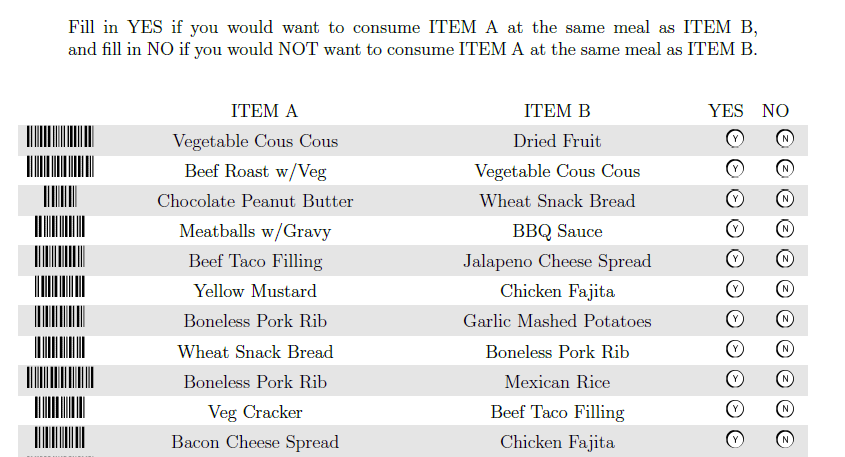
\includegraphics[width=0.9\textwidth]{./img/Figure51.png}
\end{figure}

\subsection{Data Analysis}
Due to some incomplete surveys, all pairs were evaluated between 61 and 69 times each.  Total proportions reflecting how frequently each pair was chosen as compatible were computed.  These proportions were used to create thirty-two individual lower triangular matrices, one per entr\'{e}e, as the entr\'{e}e is the centerpiece of the MRE\tm menu.  The rows and columns of these matrices corresponded to the food items in the study, with the (i,j) entry containing the compatibility proportion for the i\superscript{th} food item with the j\superscript{th} food item, according to a predetermined ordering of the items.  Where cross-category pairs were eliminated as a survey design consideration, proportions equal to 1 were input into the matrices.  All within-category pairs (e.g. Snack-Snack) were filled in with zeroes to denote these within-category pairs as incompatible and meals with multiple items from the same category impossible.

For each entr\'{e}e, we followed the following algorithm for determining the compatible meals associated with the entr\'{e}e.  The purpose of this algorithm is to determine which cutoff for compatibility we should use to define a pair of food items as “connected” from a graph theoretic standpoint.  First, we followed the following process for each of the proportion values in the matrix for the entr\'{e}e under consideration, beginning with the largest proportion and proceeding in decreasing order.  For each proportion, any smaller proportions were temporarily set to 0, meaning that the corresponding pair of food items was to be considered, for the moment, as disconnected.  Similarly, any equal or larger proportions were temporarily set to 1, meaning that the corresponding pair of food items was to be considered, for the moment, as connected.  In this temporary state, we found the cliques associated with this iteration, reset our values, and started over at the next proportion.  Recall that a clique is a fully connected combination, so in this case a clique of food items corresponds to a fully compatible meal.  As we stepped down through the proportions, we stopped our search as soon as cliques of size eight, the size of the MRE\tm menu, were found.  This approach ensured that we found the MRE\tm menus of maximum compatibility, as further relaxing our cutoff for connectedness would have yielded more, less compatible, menus.  

To evaluate the quality of these menus, we used a novel ranking approach.  Having found the fully compatible menus in our previous step, we then calculated the average proportion of compatibility for each compatible menu.  More specifically, for all inter-category pairs there was a proportion of compatibility based on the original soldier responses.  For each proposed menu, we averaged those proportions, ignoring zeroes and ones, thus providing a valuable metric for determining the best menus per entr\'{e}e.  All data analysis was conducted with R 2.10.0 and surveys were created using custom LaTeX templates and the R Sweave package.  Barcodes were used to efficiently scan in responses.

\section{Results and Discussion}
The top MRE\tm menus for each of the 32 entr\'{e}es are listed in Table~\ref{tab:mremeals}.  The score for each menu is the average proportion of compatibility between each pair that was evaluated by the soldiers for that menu.  The menu with the highest compatibility score contains Chili with Beans, with a score of 0.8160.  The  Chili with Beans menu currently in production is paired with Mexican Corn as a side, Cheese Spread and ground red pepper as a seasoning.  By replacing these items with those predicted from Table~\ref{tab:mremeals}, we expect the overall compatibility of the menu to increase along with, we predict, the overall liking of the menu.  The lowest scored menu contains Szechuan Vegetables with Tofu (score=0.6377).  This means that there was no good combination of items, from all of the possible items presented, that would create a highly compatible MRE\tm meal using this entr\'{e}e.  Rather than develop new MRE\tm menu items across the board to increase compatibility, the recommendation would be to eliminate this menu item and to focus efforts on the entr\'{e}es with medium range compatibility scores to increase compatibility and acceptance.

\begin{landscape}
\footnotesize
\begin{longtable}{p{3.0cm}p{3.7cm}p{2.2cm}p{2.0cm}p{2.3cm}p{0.8cm}p{1.5cm}p{2.2cm}p{0.8cm}}
\caption{List of No. 1 meals for each of the 32 entr\'{e}e items.  } \\
\label{tab:mremeals} \\
\endfirsthead
\midrule
{\bf Entree} & {\bf Side} & {\bf Seasoning} & {\bf Bakery} & {\bf Spreads} & {\bf Fruits} & {\bf Desserts} & {\bf Snacks} & {\bf Score}\\
\midrule
\endhead
 \multicolumn{3}{c}{Continued on next page...} \\
\endfoot
\bottomrule
\endlastfoot
\toprule
{\bf Entree} & {\bf Side} & {\bf Seasoning} & {\bf Bakery} & {\bf Spreads} & {\bf Fruits} & {\bf Desserts} & {\bf Snacks} & {\bf Score}\\
\midrule
Chili with Beans & Mex. Mac and Cheese & Herb-Citrus Seasoning & Crackers, Plain & Peanut Butter, Chunky & Fruit (Wet) & Cookies & Cheese-Filled Pretzels & 0.8160 \\
\midrule
Pork Ribs & Garlic Mashed Potatoes & Herb-Citrus Seasoning & Crackers, Plain & Peanut Butter, Chunky & Fruit (Wet) & Cookies & Cheese-Filled Pretzels & 0.8151 \\
\midrule
Beef Roast, Veg. & Cornbread Stuffing & Red Pepper & Crackers, Plain &  Peanut Butter, Chunky & Fruit (Wet) & Cookies & Cheese-Filled Pretzels & 0.8069 \\
\midrule
Buffalo Chicken & Garlic Mashed Potatoes & Red Pepper & Crackers, Plain &  Peanut Butter, Chunky & Fruit (Wet) & Cookies & Cheese-Filled Pretzels & 0.8027 \\
\midrule
Beef Taco Filling & Mexican Rice & Red Pepper & White Bread & Peanut Butter, Chocolate & Fruit (Wet) & Cookies & Cheese-Filled Pretzels & 0.8011 \\
\midrule
Chili \& Macaroni & Potato, Cheddar \& Bacon Soup & Herb-Citrus Seasoning & Crackers, Plain & Peanut Butter, Chunky & Fruit (Wet) & Cookies & Cheese-Filled Pretzels & 0.8005 \\
\midrule
Chicken Marsala & Garlic Mashed Potatoes & Hot Sauce & Crackers, Plain & Peanut Butter, Chunky & Fruit (Wet) & Cookies & Cheese-Filled Pretzels & 0.7989 \\
\midrule
Meatballs,Marinara Sauce & Potatoes au Gratin & Hot Sauce & Crackers, Plain & Peanut Butter, Chunky & Fruit (Wet) & Cookies & Cheese-Filled Pretzels & 0.7919 \\
\midrule
Beef Brisket, Gravy & Garlic Mashed Potatoes & BBQ Seasoning & Crackers, Plain & Peanut Butter, Chunky & Fruit (Wet) & Cookies & Cheese-Filled Pretzels & 0.7915 \\
\midrule
Spaghetti, Meat \& Sauce & Garlic Mashed Potatoes & Red Pepper & Crackers, Plain & Peanut Butter, Chunky & Fruit (Wet) & Cookies & Cheese-Filled Pretzels & 0.7891 \\
\midrule
Spicy Sweet \& Sour Pork & Fried Rice & Herb-Citrus Seasoning & Crackers, Plain & Peanut Butter, Chunky & Fruit (Wet) & Cookies & Cheese-Filled Pretzels & 0.7891\\
\midrule
Beef Stew & Garlic Mashed Potatoes & Red Pepper & Crackers, Plain & Peanut Butter, Smooth & Fruit (Wet) & Filled Bakery & Cheese-Filled Pretzels & 0.7869 \\
\midrule
Chicken, Tomatoes \& Feta & Fried Rice & Herb-Citrus Seasoning & Crackers, Plain & Peanut Butter, Chunky & Fruit (Wet) & Cookies & Cheese-Filled Pretzels & 0.7847 \\
\midrule
Chicken, Noodles \& Vegetables & Garlic Mashed Potatoes & Hot Sauce & Crackers, Plain & Peanut Butter, Chunky & Fruit (Wet) & Cookies & Cheese-Filled Pretzels & 0.7819 \\
\midrule
Sloppy Joe & Garlic Mashed Potatoes & Herb-Citrus Seasoning & Wheat Bread & Peanut Butter, Smooth & Fruit (Wet) & Cookies & Cheese-Filled Pretzels & 0.7810 \\
\midrule
Chicken Fajita & Mexican Rice & Herb-Citrus Seasoning & White Bread & Peanut Butter, Chocolate & Fruit (Wet) & Cookies & Cheese-Filled Pretzels & 0.7769 \\
\midrule
Meatballs in Brown Gravy & Garlic Mashed Potatoes & Herb-Citrus Seasoning & Crackers, Plain & Peanut Butter, Chunky & Fruit (Wet) & Cookies & Cheese-Filled Pretzels & 0.7753 \\
\midrule
Beef Ravioli in Meat Sauce & Garlic Mashed Potatoes & Herb-Citrus Seasoning & Crackers, Plain & Peanut Butter, Chunky & Fruit (Wet) & Cookies & Cheese-Filled Pretzels & 0.7722 \\
\midrule
Beef Patty, Pepper Jack & Potatoes au Gratin & BBQ Sauce & Wheat Bread & Peanut Butter, Smooth & Fruit (Wet) & Cookies & Cheese-Filled Pretzels & 0.7719 \\
\midrule
Cheese Tortellini in Tomato Sauce & Potato, Cheddar \& Bacon Soup & Red Pepper & Crackers, Plain & Peanut Butter, Chunky & Fruit (Wet) & Cookies & Cheese-Filled Pretzels & 0.7657 \\
\midrule
Turkey Chili with Hominy & Garlic Mashed Potatoes & Hot Sauce & Crackers, Plain & Peanut Butter, Chunky & Fruit (Wet) & Cookies & Cheese-Filled Pretzels & 0.7596 \\
\midrule
Tuna with Lemon Pepper & Garlic Mashed Potatoes & Herb-Citrus Seasoning & Crackers, Plain & Peanut Butter, Chunky & Fruit (Wet) & Cookies & Cheese-Filled Pretzels & 0.7574 \\
\midrule
Mex. Chicken Stew & Mex. Mac and Cheese & Hot Sauce & Crackers, Plain & Peanut Butter, Chunky & Fruit (Wet) & Cookies & Cheese-Filled Pretzels & 0.7570 \\
\midrule
Pork Sausage with Gravy & Garlic Mashed Potatoes & Herb-Citrus Seasoning & Crackers, Plain & Peanut Butter, Chunky & Fruit (Wet) & Cookies & Cheese-Filled Pretzels & 0.7531 \\
\midrule
Southwest Beef \& Black Beans & Fried Rice & Hot Sauce & Crackers, Plain & Peanut Butter, Chunky & Fruit (Wet) & Cookies & Cheese-Filled Pretzels & 0.7422 \\
\midrule
Chicken Pesto Pasta & Garlic Mashed Potatoes & Herb Citrus Seasoning & Multigrain Bread & Peanut Butter, Chunky & Fruit (Wet) & Cookies & Cheese-Filled Pretzels & 0.7416 \\
\midrule
Vegetable Lasagna & Potatoes au Gratin & Hot Sauce & Crackers, Plain & Peanut Butter, Chunky & Fruit (Wet) & Cookies & Cheese-Filled Pretzels & 0.7391 \\
\midrule
Penne with Sausage, Spicy Tomato Sauce & Garlic Mashed Potatoes & Red Pepper, Ground & Vegetable Crackers & Peanut Butter, Chunky & Fruit (Wet) & Cookies & Cheese-Filled Pretzels & 0.7360 \\
\midrule
Ratatouille & Garlic Mashed Potatoes & Red Pepper & Crackers, Plain & Peanut Butter, Chunky & Fruit (Wet) & Cookies & Cheese-Filled Pretzels & 0.7301 \\
\midrule
Pork Sausage Patty, Maple Flavored & Granola & Table Syrup & Wheat Bread & Peanut Butter, Smooth & Fruit (Wet) & Cookies & Cheese-Filled Pretzels & 0.7281 \\
\midrule
Maple Sausage Wrap & Granola & Table Syrup & Multigrain Bread & Peanut Butter, Chunky & Fruit (Wet) & Cookies & Cheese-Filled Pretzels & 0.7100 \\
\midrule
Szechuan Vegetables \& Tofu & Fried Rice & Herb Citrus Seasoning & Vegetable Crackers & Peanut Butter, Chunky & Fruit (Wet) & Cookies & Cheese-Filled Pretzels & 0.7377 \\
\end{longtable}
\end{landscape}

There were two entr\'{e}e items that were being considered for introduction.  Field tests to evaluate the palatability of the new entr\'{e}es typically are challenging, because the development group, by necessity, would make educated guesses as to which of the other meal items they should pair with the entr\'{e}e to create the MRE\tm meal.  We know that flavor contrast effects and other contextual effects are important to our overall concept of the meal, so it is important to choose the entire meal carefully.  Our study incorporated the two new entr\'{e}es, which were the Beef Patty and the Beef Taco Filling.  The best predicted menus are shown in Table~\ref{tab:mremeals}.  Both menus have strong meal proportion scores, and the Beef Taco Filling is one of only six entr\'{e}es with a score above 0.80.  This gives evidence that this particular meal combination is likely to be highly successful.  

Table~\ref{tab:mrechili} contains the top 10 MRE\tm menus for the Chili Mac entr\'{e}e.  This table illustrates the value of this approach as a screening tool and not as an ultimate solution providing a single answer.  For example, in Table~\ref{tab:mremeals} we notice that there is very little variation in some of the categories, such as Desserts and Spreads.  However, using Table~\ref{tab:mrechili} we can see that we could use the 8th ranked combination rather than the 1st ranked item, introduce some variety into this category, and the compatibility score drops only 0.50\%.  

\begin{landscape}
\footnotesize
\begin{longtable}{p{0.5cm}p{4cm}p{4cm}p{2cm}p{2.3cm}p{0.8cm}p{1.5cm}p{2.2cm}p{0.8cm}}
\caption{Top 10 menus for the Chili-mac entree item } \\
\label{tab:mrechili}
\endfirsthead
\midrule
{\bf Rank} & {\bf Side} & {\bf Seasoning} & {\bf Bakery} & {\bf Spreads} & {\bf Fruits} & {\bf Desserts} & {\bf Snacks} & {\bf Score}\\
\hline
\endhead
\multicolumn{3}{c}{Continued on next page...} \\
\endfoot
\bottomrule
\endlastfoot
\toprule
{\bf Rank} & {\bf Side} & {\bf Seasoning} & {\bf Bakery} & {\bf Spreads} & {\bf Fruits} & {\bf Desserts} & {\bf Snacks} & {\bf Score}\\
\midrule
1 & Potato, Cheddar \& Bacon Soup & Herb-Citrus Seasoning & Crackers, Plain & Peanut Butter, Chunky & Fruit (Wet) & Cookies & Cheese-filled Pretzels & 0.8005\\
\midrule
2 & Potato, Cheddar \& Bacon Soup & Herb-Citrus Seasoning & Wheat Bread & Peanut Butter, Chocolate & Fruit (Wet) & Cookies & Cheese-filled Pretzels & 0.7988\\
\midrule
3 & Potato, Cheddar \& Bacon Soup & Red Pepper & Crackers, Plain & Peanut Butter, Chunky & Fruit (Wet) & Cookies & Cheese-filled Pretzels & 0.7975\\
\midrule
4 & Potato, Cheddar \& Bacon Soup & Herb-Citrus Seasoning & Crackers, Plain & Cheese Spread, Plain & Fruit (Wet) & Cookies & Cheese-filled Pretzels & 0.7973\\
\midrule
5 & Potato, Cheddar \& Bacon Soup & Herb-Citrus Seasoning & Crackers, Plain & Peanut Butter, Chunky & Fruit (Wet) & Filled Bakery & Cheese-filled Pretzels & 0.7968\\
\midrule
\\
\\
\\
\\

6 & Potato, Cheddar \& Bacon Soup & Herb-Citrus Seasoning & Wheat Bread & Jelly or Jam & Fruit (Wet) & Cookies & Cheese-filled Pretzels & 0.7968\\
\midrule
7 & Potato, Cheddar \& Bacon Soup & Red Pepper & Wheat Bread & Peanut Butter, Chocolate & Fruit (Wet) & Cookies & Cheese-filled Pretzels & 0.7955\\
\midrule
8 & Potato, Cheddar \& Bacon Soup & Herb-Citrus Seasoning & Wheat Bread & Peanut Butter, Chocolate & Fruit (Wet) & Filled Bakery & Cheese-filled Pretzels & 0.7943\\
\midrule
9 & Potato, Cheddar \& Bacon Soup & Red Pepper & Crackers, Plain & Cheese Spread, Plain & Fruit (Wet) & Cookies & Cheese-filled Pretzels & 0.7943\\
\midrule
10 & Potato, Cheddar \& Bacon Soup & Herb-Citrus Seasoning & Crackers, Plain & Cheese Spread, Plain & Fruit (Wet) & Filled Bakery & Cheese-filled Pretzels & 0.7942\\
\end{longtable}
\end{landscape}

In a similar vein and perhaps unsurprisingly since the respondents were a typical cross-section of soldiers, some of the entr\'{e}es that are designated vegetarian have been combined with meat based side items (e.g. Penne with Vegetables and Potato, Cheddar and Bacon soup).  This is another example where the expertise of the meal developers is critical to find and further screen out these incompatible combinations.  Alternatively, this expertise could be used to further restrict the pairs included in the test design, in this case not presenting soldiers with any pairs involving vegetarian and non-vegetarian items simultaneously.  Other restrictions specific to MREs\tm that are not incorporated into the model and are left for screening include size of components, nutritional restrictions, variety  and intended use.  It is worth noting that tools from discrete mathematics, specifically algorithms that approach the so-called “knapsack” problem could be used to address these problems \citep{Martello1990}.  As currently executed, however, the current proposed meal development approach provides an excellent tool for evaluating and screening billions of potential meals.

One possibility worthy of investigation is that compatibility scores  might be correlated with whether or not a menu item is liked at all.  That is, if an item is compatible with large numbers of other items, it may well be a highly liked item.  Alternatively, an item with low compatibility with other items, e.g. the Szechuan Vegetables with Tofu item, in the present study might well be simply a disliked item and no combination at all would make the score of this entr\'{e}e high.  A useful follow-up study could investigate these correlations.  If there is liking information embedded in the compatibility information, this approach would prove even more powerful.

With the addition of categories to the \citet{Ennisa} model, we have provided a way to measure complex information about meal experience.  This methodology takes a meta-level approach to meal design by looking at which items are combined together most often using the consumers, in this case soldiers, themselves to define the criteria for connectivity.  As long as consumers have some sort of common understanding of what should be combined together, no matter the reason, this methodology will capture compatibility patterns and provide concrete recommendations for highly compatible menus.  Even though this approach does not specifically concern itself with the social, psychological and nutritional factors that \citet{Meiselman2000} proposes as building blocks of the meal experience, by incorporating the graph theoretic approach with an appropriateness framework and internal expertise, all three of Meiselman’s factors are accounted for.  	

\section{Acknowledgements}
We thank Daniel Ennis and Charles Fayle for their support, ideas and expertise in the execution of this investigation.

\pagebreak
\renewcommand\bibname{{REFERENCES}} %  will print "REFERENCES" instead of "BIBLIOGRAPHY"
\phantomsection
\addcontentsline{toc}{section}{References} %  adds "REFERENCES" to the table of content
\bibliographystyle{apalike}
\bibliography{library_man}  % uses the references stored in Chapter1Radar.bib